\hypertarget{camera}{%
\section{Camera}\label{camera}}

This project contains the interface \textbf{Camera} for all cameras. The
actual implementations are: IDS.

\textbf{Requirements}

\includegraphics{https://img.shields.io/static/v1?label=cpp\&message=11\&color=007bff}

\includegraphics{https://img.shields.io/static/v1?label=cmake\&message=3.16\&color=007bff}

\includegraphics{https://img.shields.io/static/v1?label=git\&message=2.0\&color=007bff}

\includegraphics{https://img.shields.io/static/v1?label=Doxygen\&message=1.8.13\&color=007bff}

\includegraphics{https://img.shields.io/static/v1?label=Sphinx\&message=3.0.2\&color=007bff}

\includegraphics{https://img.shields.io/static/v1?label=OS\&message=Win\&color=28a745\%22}

\hypertarget{generality}{%
\subsection{Generality}\label{generality}}

\hypertarget{import}{%
\subsubsection{Import}\label{import}}

Import as an external library into your project by copy-paste the
following lines in your \texttt{config.json}.

\begin{Shaded}
\begin{Highlighting}[]
\FunctionTok{\{}
  \DataTypeTok{"name"}     \FunctionTok{:} \StringTok{"PATCamera"}\FunctionTok{,}
  \DataTypeTok{"path"}     \FunctionTok{:} \StringTok{"gitlab.dei.unipd.it/PAT/Camera.git"}\FunctionTok{,}
  \DataTypeTok{"tag"}      \FunctionTok{:} \StringTok{"HEAD"}\FunctionTok{,}
  \DataTypeTok{"available"}\FunctionTok{:} \StringTok{"YES"}\FunctionTok{,}
  \DataTypeTok{"getGui"}   \FunctionTok{:} \StringTok{"YES"}
\FunctionTok{\}}
\end{Highlighting}
\end{Shaded}

\hypertarget{prerequisites}{%
\subsubsection{Prerequisites}\label{prerequisites}}

The following libraries are auto fetched from the gitlab.dei.unipd.it
host (ask the owner of this repo to become a member):

\begin{itemize}
\tightlist
\item
  \href{https://gitlab.dei.unipd.it/PAT/Centroid.git}{Centroid} 1.0.0
\end{itemize}

These other libraries need to be installed manually in your system:

\begin{itemize}
\tightlist
\item
  \href{https://www.qt.io/}{Qt} 5.14.2
\end{itemize}

The library documentation is generated through
\href{http://www.doxygen.nl/download.html}{Doxygen 1.8.13}. Additional
documentation in the \texttt{index} folder is generated through the
\href{https://www.anaconda.com/products/individual}{python3} package
\href{https://www.sphinx-doc.org/en/master/}{Sphinx} using the following
extensions (which you can install through pip3):

\begin{itemize}
\tightlist
\item
  \href{https://pypi.org/project/Sphinx/}{Sphinx 3.0.2}
\item
  \href{https://sphinx-rtd-theme.readthedocs.io/en/stable/}{Sphinx read
  the doc theme} (to use the read the doc theme for html documentation)
\item
  \href{https://pypi.org/project/breathe/}{Breathe} (to use the xml
  output of doxygen)
\item
  \href{https://pypi.org/project/sphinx-markdown-builder/}{Sphinx-markdown-builder}
  (to generate the markdown version for gitlab wiki)
\end{itemize}

\texttt{pip3\ install\ Sphinx\ sphinx\_rtd\_theme\ breathe\ sphinx-markdown-builder}

\hypertarget{usage}{%
\subsection{Usage}\label{usage}}

\hypertarget{frame}{%
\subsubsection{Frame}\label{frame}}

The \textbf{Frame} class manages all the processing of the images
captured by the camera.

\begin{Shaded}
\begin{Highlighting}[]
\PreprocessorTok{\#include }\ImportTok{\textless{}PAT/Camera/Frame.h\textgreater{}}
\end{Highlighting}
\end{Shaded}

This is an example of initialization.

\begin{Shaded}
\begin{Highlighting}[]
\DataTypeTok{int}\NormalTok{ width = }\DecValTok{100}\NormalTok{;}
\DataTypeTok{int}\NormalTok{ height = }\DecValTok{100}\NormalTok{;}
\DataTypeTok{unsigned} \DataTypeTok{char}\NormalTok{ imgBuffer[width * height] = \{}\DecValTok{0}\NormalTok{\};}
\BuiltInTok{std::}\NormalTok{shared\_ptr\textless{}Frame\textgreater{} frame = }\BuiltInTok{std::}\NormalTok{make\_shared\textless{}Frame\textgreater{}(imgBuffer, width, height, }\ExtensionTok{QImage::}\NormalTok{Format\_Grayscale8);}
\end{Highlighting}
\end{Shaded}

You can flip the image in the two axes usign these functions.

\begin{Shaded}
\begin{Highlighting}[]
\NormalTok{frame{-}\textgreater{}flipX();}
\NormalTok{frame{-}\textgreater{}flipY();}
\end{Highlighting}
\end{Shaded}

You can calculate the centroid, the spotDiameter and the integral (spot
intensity) using this function. If it does not find the centroid it
returns -1 as invalid value.

\begin{Shaded}
\begin{Highlighting}[]
\NormalTok{frame{-}\textgreater{}calculateCentroidAndIntegral();}
\end{Highlighting}
\end{Shaded}

You can also control the centroid calculation setting the parameters
\textbf{threshold} and \textbf{rangeRadius}. -
\textbf{setThreshold/getThreshold} set/get the minimum value for pixels
to be counted in the centroid average. -
\textbf{setRangeRadius/getRangeRadius} set/get the range radius in pixel
where to search the centroid. The value 0 means infinite range. -
\textbf{getRange} get the four cordinate of the range where to search
the centroid.

\begin{Shaded}
\begin{Highlighting}[]
\KeywordTok{auto}\NormalTok{ threshold = frame{-}\textgreater{}getThreshold();}
\NormalTok{threshold.value = }\DecValTok{30}\NormalTok{;}
\NormalTok{frame{-}\textgreater{}setThreshold(threshold);}

\KeywordTok{auto}\NormalTok{ rangeRadius = frame{-}\textgreater{}getRangeRadius();}
\NormalTok{rangeRadius.value = }\DecValTok{200}\NormalTok{;}
\NormalTok{frame{-}\textgreater{}setRangeRadius(rangeRadius);}

\NormalTok{PAT::Utils::Range\textless{}}\DataTypeTok{int}\NormalTok{\textgreater{} range = frame{-}\textgreater{}getRange()}
\end{Highlighting}
\end{Shaded}

You can get the other parameters using these functions.

\begin{Shaded}
\begin{Highlighting}[]
\BuiltInTok{std::}\NormalTok{shared\_ptr\textless{}PAT::Centroid\textgreater{} centroid = frame{-}\textgreater{}getCentroid();}
\BuiltInTok{std::}\NormalTok{shared\_ptr\textless{}PAT::Utils::BoundedParameter\textless{}PAT::Utils::Circle\textless{}}\DataTypeTok{int}\NormalTok{\textgreater{}\textgreater{}\textgreater{} target = frame{-}\textgreater{}getTarget();}
\DataTypeTok{unsigned} \DataTypeTok{char}\NormalTok{* imgBuffer = frame{-}\textgreater{}getImageRaw();}
\ExtensionTok{QImage}\NormalTok{ img = frame{-}\textgreater{}getImage();}
\DataTypeTok{int}\NormalTok{ width = frame{-}\textgreater{}getWidth();}
\DataTypeTok{int}\NormalTok{ height = frame{-}\textgreater{}getHeight();}
\end{Highlighting}
\end{Shaded}

\hypertarget{camera-1}{%
\subsubsection{Camera}\label{camera-1}}

The \textbf{Camera} class is a interface for all Camera. Here is the
include code.

\begin{Shaded}
\begin{Highlighting}[]
\PreprocessorTok{\#include }\ImportTok{\textless{}PAT/Camera/Camera.h\textgreater{}}
\end{Highlighting}
\end{Shaded}

To inherit the class you have to overwrite the four methods:
\textbf{start}, \textbf{stop}, \textbf{setFrameRate},
\textbf{setExposureTime}.

\begin{Shaded}
\begin{Highlighting}[]
\KeywordTok{class}\NormalTok{ YourClass : }\KeywordTok{public}\NormalTok{ Camera \{}
\KeywordTok{public}\NormalTok{:}
  \DataTypeTok{void}\NormalTok{ start() }\KeywordTok{override}\NormalTok{;}
  \DataTypeTok{void}\NormalTok{ stop() }\KeywordTok{override}\NormalTok{;}
  \DataTypeTok{void}\NormalTok{ setFrameRate(}\AttributeTok{const}\NormalTok{ PAT::Utils::BoundedParameter\textless{}}\DataTypeTok{double}\NormalTok{\textgreater{}\& \_frameRate) }\KeywordTok{override}\NormalTok{;}
  \DataTypeTok{void}\NormalTok{ setExposureTime(}\AttributeTok{const}\NormalTok{ PAT::Utils::BoundedParameter\textless{}}\DataTypeTok{double}\NormalTok{\textgreater{}\& \_exposureTimeValue) }\KeywordTok{override}\NormalTok{;}
\NormalTok{\};}
\end{Highlighting}
\end{Shaded}

\hypertarget{ids}{%
\subsubsection{IDS}\label{ids}}

The \textbf{IDS} class is a Camera implementation. Here is the include
code.

\begin{Shaded}
\begin{Highlighting}[]
\PreprocessorTok{\#include }\ImportTok{\textless{}PAT/Camera/IDS.h\textgreater{}}
\KeywordTok{using} \KeywordTok{namespace}\NormalTok{ PAT::Camera;}
\end{Highlighting}
\end{Shaded}

The \textbf{IDS} is typically used as polymorphism with \textbf{Camera}.
In order to define a variable you can choose to pass the \textbf{IDS id}
or to let it automatically search it. If the search fails the program
throw an exception "not found". To search the id you can use
\textbf{find} and \textbf{findAll} functions.

\begin{Shaded}
\begin{Highlighting}[]
\BuiltInTok{std::}\NormalTok{shared\_ptr\textless{}PAT::Camera::Camera\textgreater{} camera = }\BuiltInTok{std::}\NormalTok{make\_shared\textless{}PAT::Camera::IDS\textgreater{}();}
\BuiltInTok{std::}\NormalTok{shared\_ptr\textless{}PAT::Camera::Camera\textgreater{} camera = }\BuiltInTok{std::}\NormalTok{make\_shared\textless{}PAT::Camera::IDS\textgreater{}(IDS::find());}
\BuiltInTok{std::}\NormalTok{shared\_ptr\textless{}PAT::Camera::Camera\textgreater{} camera = }\BuiltInTok{std::}\NormalTok{make\_shared\textless{}PAT::Camera::IDS\textgreater{}(IDS::findAll(){-}\textgreater{}uci[}\DecValTok{0}\NormalTok{].dwCameraID);}
\end{Highlighting}
\end{Shaded}

You can enable/disable or check if enabled the IDS's acquisition using
these functions.

\begin{Shaded}
\begin{Highlighting}[]
\ControlFlowTok{if}\NormalTok{(!camera{-}\textgreater{}isActive())}
\NormalTok{ camera{-}\textgreater{}start();}
\ControlFlowTok{else}
\NormalTok{ camera{-}\textgreater{}stop();}
\end{Highlighting}
\end{Shaded}

You can set the frame rate of the acquisition using these functions. At
every frame the Camera calculates the centroid and then it emit a signal
\textbf{newFrameSignal}.

\begin{Shaded}
\begin{Highlighting}[]
\KeywordTok{auto}\NormalTok{ framerate  = camera{-}\textgreater{}getFrameRate();}
\NormalTok{framerate.value = }\DecValTok{30}\NormalTok{;}
\NormalTok{camera{-}\textgreater{}setFrameRate(framerate);}
\end{Highlighting}
\end{Shaded}

You can set the exposure time of the acquisition using these functions.
The exposure time limit depends on the frame rate (1 / framerate).

\begin{Shaded}
\begin{Highlighting}[]
\KeywordTok{auto}\NormalTok{ exposureTime  = camera{-}\textgreater{}getExposureTime();}
\NormalTok{exposureTime.value = }\DecValTok{1}\NormalTok{ / }\DecValTok{30}\NormalTok{;}
\NormalTok{camera{-}\textgreater{}setExposureTime(exposureTime);}
\end{Highlighting}
\end{Shaded}

You can enable/disable or check if enabled the centroid calculation
using these functions.

\begin{Shaded}
\begin{Highlighting}[]
\ControlFlowTok{if}\NormalTok{(!camera{-}\textgreater{}getCentroidCalculation())}
\NormalTok{ camera{-}\textgreater{}setCentroidCalculation(}\KeywordTok{true}\NormalTok{);}
\ControlFlowTok{else}
\NormalTok{ camera{-}\textgreater{}setCentroidCalculation(}\KeywordTok{false}\NormalTok{);}
\end{Highlighting}
\end{Shaded}

You can alse obtain the frame object that it automatically update at
every frame.

\begin{Shaded}
\begin{Highlighting}[]
\BuiltInTok{std::}\NormalTok{shared\_ptr\textless{}Frame\textgreater{} frame = camera{-}\textgreater{}getFrame();}
\end{Highlighting}
\end{Shaded}

\hypertarget{camerawiget}{%
\subsubsection{CameraWiget}\label{camerawiget}}

The \textbf{CameraWiget} class is a widget fot the Camera's
implementations. Here I present the IDS example. The include code is the
following.

\begin{Shaded}
\begin{Highlighting}[]
\PreprocessorTok{\#include }\ImportTok{\textless{}QApplication\textgreater{}}
\PreprocessorTok{\#include }\ImportTok{\textless{}PAT/Camera/gui/CameraWidget.h\textgreater{}}
\PreprocessorTok{\#include }\ImportTok{\textless{}PAT/Camera/IDS.h\textgreater{}}
\KeywordTok{using} \KeywordTok{namespace}\NormalTok{ PAT::Camera;}
\end{Highlighting}
\end{Shaded}

This is a simple \textbf{main} example.

\begin{Shaded}
\begin{Highlighting}[]
\DataTypeTok{int}\NormalTok{ main(}\DataTypeTok{int}\NormalTok{ argc, }\DataTypeTok{char}\NormalTok{ *argv[]) \{}
  \ExtensionTok{QApplication}\NormalTok{ a(argc, argv);}
\NormalTok{  CameraWidget cameraWidget;}
  \BuiltInTok{std::}\NormalTok{shared\_ptr\textless{}Camera\textgreater{} camera = }\BuiltInTok{std::}\NormalTok{make\_shared\textless{}IDS\textgreater{}();}
\NormalTok{  cameraWidget.setCamera(camera);}
\NormalTok{  cameraWidget.show();}
\NormalTok{  camera{-}\textgreater{}start();}
 \ControlFlowTok{return}\NormalTok{ a.exec();}
\NormalTok{\}}
\end{Highlighting}
\end{Shaded}

If you want instead integrate the widget into another GUI (layout) you
can use this code.

\begin{Shaded}
\begin{Highlighting}[]
\ExtensionTok{QWidget}\NormalTok{ *window                = }\KeywordTok{new} \ExtensionTok{QWidget}\NormalTok{();}
\ExtensionTok{QVBoxLayout}\NormalTok{ *mainLayout        = }\KeywordTok{new} \ExtensionTok{QVBoxLayout}\NormalTok{();}
\NormalTok{CameraWidget *cameraWidget     = }\KeywordTok{new}\NormalTok{ CameraWidget();}
\BuiltInTok{std::}\NormalTok{shared\_ptr\textless{}Camera\textgreater{} camera = }\BuiltInTok{std::}\NormalTok{make\_shared\textless{}IDS\textgreater{}();}

\NormalTok{cameraWidget{-}\textgreater{}setCamera(camera);}
\NormalTok{mainLayout{-}\textgreater{}addWidget((}\ExtensionTok{QWidget}\NormalTok{ *)cameraWidget);}
\NormalTok{window{-}\textgreater{}setLayout(mainLayout);}
\NormalTok{window{-}\textgreater{}show();}
\end{Highlighting}
\end{Shaded}

\hypertarget{uml}{%
\subsection{UML}\label{uml}}

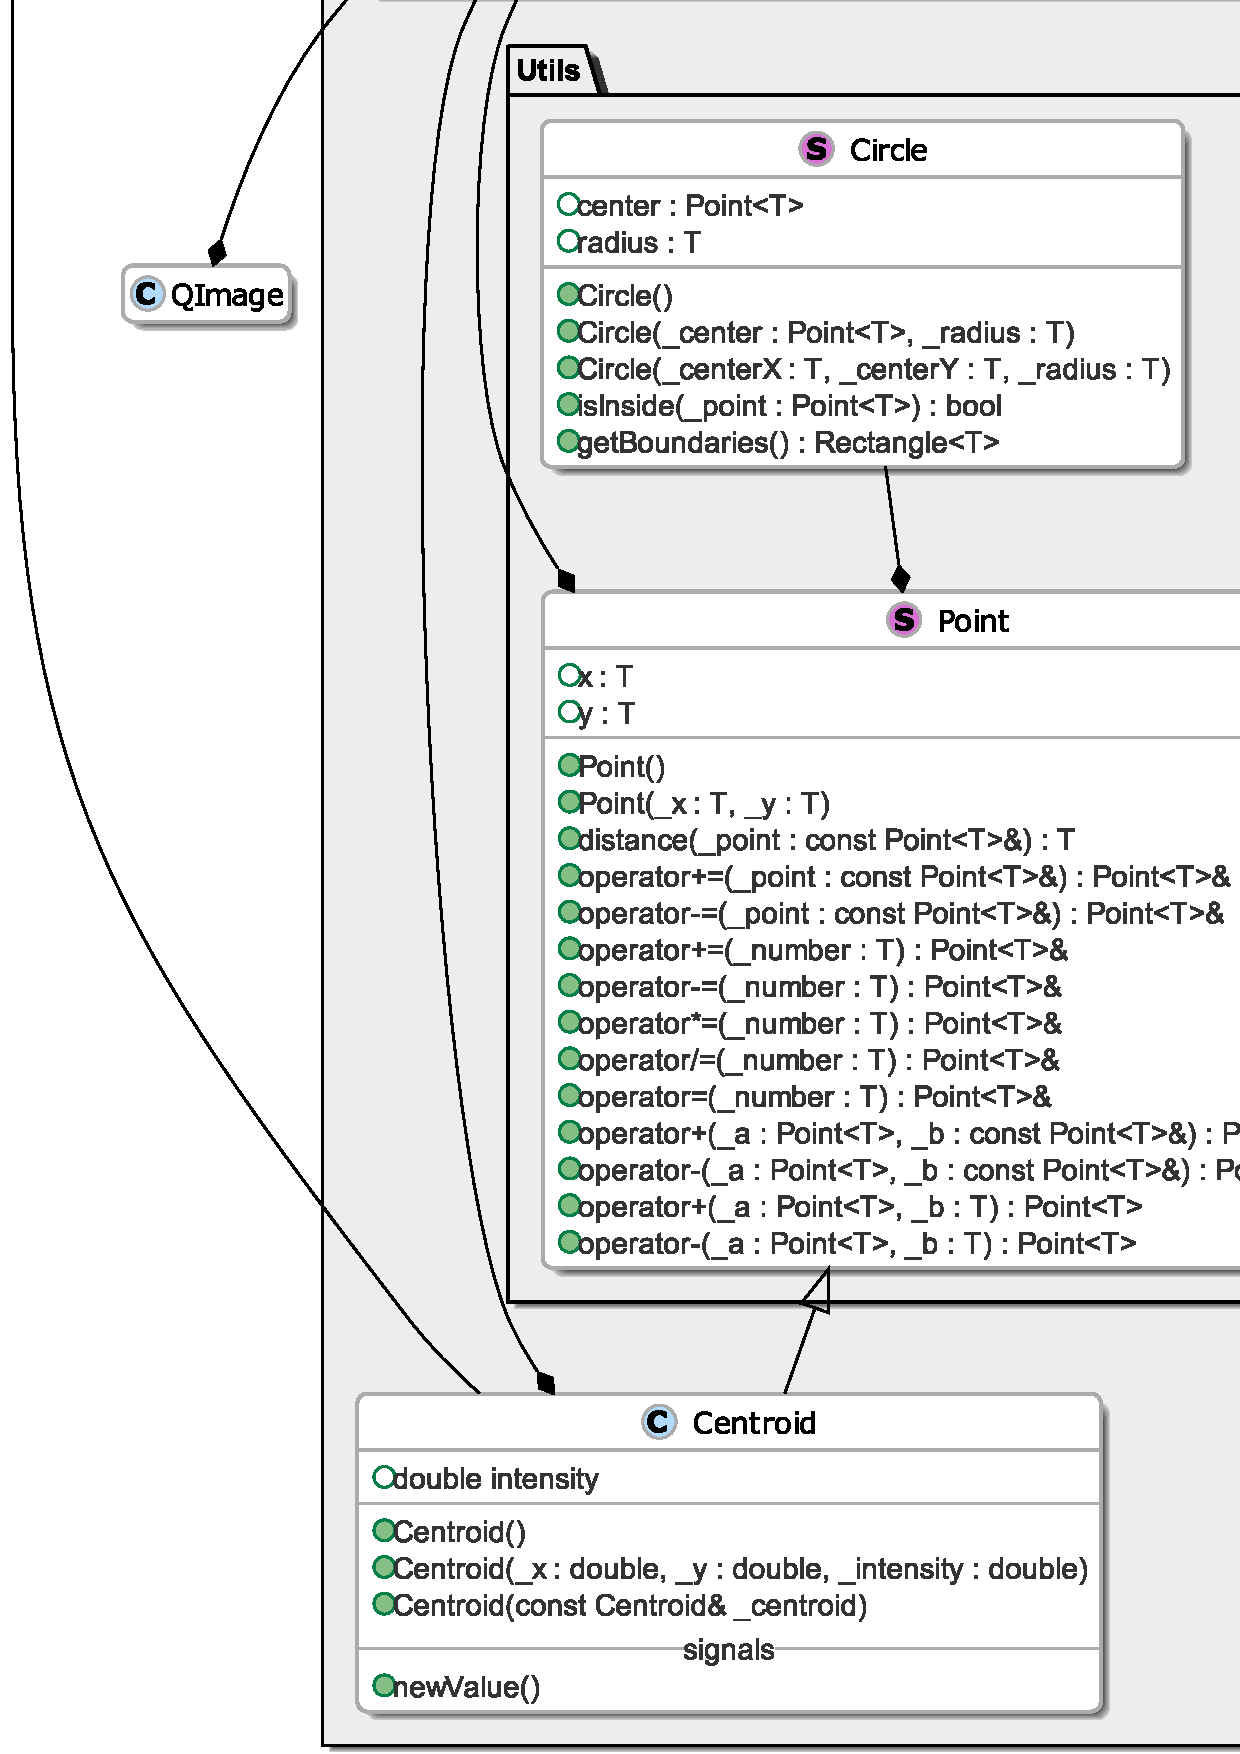
\includegraphics[width=8.33333in,height=\textheight]{https://gitlab.dei.unipd.it/pat/docs/-/raw/4da37d1e14c960824565fc73d9bca1143e667907/out/repositories/Camera/Camera.svg}
